\subsection{August 13, 2008}
\subsubsection*{The Background}
I've been feeling pretty pessimistic lately.  Andrew still weighs
heavily on my mind, and I'm finding out slowly just how deeply I had
entrenched him into my life.  I was really pretty torn up when he left
me, and everything was made worse when I found out that he did so simply
to be with someone he was already nearly dating behind my back.  Last
night, however, I found out that they were \emph{moving} in together in New
York, despite all his plans to \emph{move} out with me in Colorado.  Feeling
deeply hurt, I stopped watching his journal, and blocked him from
communicating directly with me.  I had done my best to wish them luck, and
now I feel as if I'm just having my nose rubbed in the ruins of our
relationship, so I'm breaking off all contact.  I'm telling myself that
I need to do this in order to get over him and \emph{move} on with the rest of my
life, but really, I'm sure it's little more than a passive aggressive
way for me to get back at him for telling me he'd keep in touch and then
doing this.

All of this seems rather petty in light of my growing feelings for
James, and the concerns I have with him now.  That he \emph{moved}
away from me shortly after we got together certainly isn't helping
things.  It's not the reasons that he \emph{moved} that bother me, of
course, simply that, after my previous relationships, adding that extra
element of distance makes me very, very nervous for the future of this
one, even if it's only down to denver.  I can hardly \emph{move} down 
to join him until I'm finished with school, too.

Finally, the added financial burden of my own tuition is beginning to
worry me a good deal more.  I seem to be \emph{stuck} in this
ceaseless cycle of sleeping in too late and spending all the money I
make on things I don't really need, whereas I really shouldn't let my
wants \emph{hinder} my needs.  I may want that new rifle, but I need
to finish school!

All this pessimism has served to do little more than \emph{block} my
creativity.  I have written only about 30 measures of real music this
summer, as the weight of my emotions keeps \emph{forcing me to stop}
before I feel like I've accomplished much.

As may be evident, I'm having a real problem with \emph{movement} and
the \emph{inability to move}.  I feel stopped up in many ways, as if
the world --- particularly those close to me --- race on by without me.
And so I laid out the cards\ldots

\subsubsection*{The Drawing}
With my dark mood, I chose Aleister Crowley's
\textbf{Thoth}\cite{tarotThoth} deck to do the
reading, figuring that the bright and attractive colors of the RWS deck
didn't quite match what I was feeling.  I wasn't feeling simply down,
either, or I might've chosen the Aquarian deck for its dreary, clouded
look.  I wanted the sharp, geometric shapes and smart color choices of
Lady Frieda Harris' cards to fill out my mood.

I shuffled and shuffled and shuffled until I finally felt I was ready,
and then went through the process of drawing the cards shown to me so
long ago.  Since my emotions where seemingly holding up my life, looking
for resolution, I let them choose the cards, fanning them between my two
hands until I felt that little tug at my subconscious, saying `draw that
card!'.  My intellect continued to take the back seat as my fingers
arranged the cards, face down, into the pattern that I thought they
would best fit when flipped, and for the most part, they chose well.

The pattern started with a card in the upper left, leftmost of a row of
three cards that moved down and to the right.  Directly above the last
card and in line with the leftmost card was another, and directly to the
right of that was a card with another one overlapping the upper-right
hand corner.

From left to right, the cards were:
\begin{itemize}
  \item 6 of Wands, `Victory'
  \item Queen of Disks
  \item 5 of Wands, `Strife'
  \item Above the previous card, 6 of Swords, `Science'
  \item To the right of the previous card, Princess of Swords
  \item Overlapping the upper-right hand corner of the previous card, 4
  of Wands, `Completion'
\end{itemize}
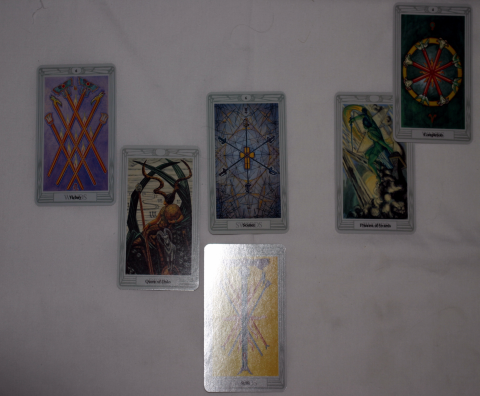
\includegraphics{image8-13-08.png}

\subsection*{The Reading}
The theme of movement became more and more evident as the cards were
flipped over, one by one, starting from the left of the board.  Wands
is the suit of fire, that which is never still.  If nothing else, fire
moves downwards and outwards as it consumes, while air, water, and earth
can all be relatively motionless.  

While the wands start out as a roaring bonfire of problems, the dwindle 
down toward the Ace to the quiet glow of a candle's flame, and the six 
is right when things begin to turn towards calm.  As was mentioned
before, fire moves downwards as it consumes, and, in fact, the first
thing that I noticed about this card was that the small flames in the
vertices of six crossed wands look as if they're forming an arrow
pointing downwards, or else that they're small concerns settling down to
the bottom of the container, relaxing.  This, I feel, is what I may be
going through now.  Despite the problems it caused me, the recent break
up is starting to become less pertinent, I am learning to deal with
James' new distance, and I do see that it is possible for me to pay my
tuition.

Taking this as my cue, I turned over the next card to the right and
slightly lower than the six, revealing the Queen of disks.  Of all of
the cards in the Thoth deck, this one is my favorite.  Many of the minor
arcana cards are little more than pip cards, and most of the court cards
of other suits are dynamic, busy images, whereas the Queen of disks sits
serenely.  Hers is the knowledge of magic of nature, and she sits
ensconced in her angular fronds, looking out over a dry valley with a
snaking river.  This, I think, is the very description of peace in
wisdom.  She is content in life, but not uncomfortable without, a
balance of emotional and intellect that echos through all of the disks.
This card shows me what I've wanted to be ever since I saw it, and I
feel that I'm starting to settle towards it, getting closer to that
ideal.

I turned over the two cards next to it at the same time, as they were in
the same vertical plane.  This revealed two more cards of movement.  The
Golden Dawn (the society of which Crowley was a member, and the source
of inspiration for this deck) label for the lower card is strife, but not
only does the card not give the impression of strife, but the other
common interpretation gives a different impression, as well: that of
striving.  The 5 of wands is a card of battle, but the card of discourse and
games, where there is action, even against another person, but
purposefu and with rules, not unfair, uncivil acts of strife against
another.  Its lower indication indicated to me the subconscious or
unconscious, showing me how my emotions where striving against each
other and against me, but that it was fair, there was a reason, and that
its not strife without rules.

The upper card, the more conscious of the two, is in elemental
opposition to the Queen of disks.  That is, swords and disks, air and
earth, do not mix well, and this alters the meaning of the cards,
bringing out the darker side of both the Queen and this, the 6 of
swords.  It shows that, while the Queen may be comfortable with the idea
of that lifeless desert behind her, she remains forever ensconced in
the life-filled oasis.  To apply the analogy, I may find the idea of
that barren desert of completely settled emotions perfectly acceptable,
but I'm too caught up in my ways, too blinded by intellect,
internalization, and change to let my emotions settle down --- I may
internalize a lot of things, but I'm letting that hinder myself as the
world changes around me.

The Six of swords itself is another card of movement, but rather than
physical movement, this is the movement of an idea or emotion through
time, such as the path that mourning takes.  Something isn't quite right
with the path as it is, though, with the influence of the Queen: the
swords are the suit of silence, and that has me stuck.  Having to take
all of this emotion from the breakup into myself without saying anything
is damaging the way I move through my life, hindering that necessary
passage of mourning while keeping the emotion smoldering.  This shows
the need for communication and action --- the card being above that
subconscious five suggests its more conscious and active role --- in
order to help these issues resolve themselves.

So what about the last two cards?  I turned them over to find the Four
of wands covering the corner of the Princess of swords.  The Princess of
swords, as the earthy side of air, shows the fixation of the volatile,
the ideas made real (she even wears the visage of Medusa on her helmet).
This, to me, was a strong suggestion that I needed to apply my ideas, to
bring them to fruition.  All of the cards before me were giving me a
path and this was saying that, if I followed that path and brought it to
reality, it would be the basis for the card that was above and
overlapping the Princess, the Four of wands, labeled `Completion'. 

More than simply the end of a process, this card shows integration.  The
four wands form a square, their points form an octagon, they are bound
in a circle, everything is integrated.  This is not saying ``Do these
things and everything will magically be resolved,'' this is saying
``Everything was, is, and will be interconnected, forever.''  If I look
to change myself, something else connected to me will change; if I move
forward in my life, I will move forward with a whole host of
opportunities and emotions.  I have always been `complete', whether or
not I have a problem, and I'm certainly realistic enough to realize that
as soon as these problems are resolved, a new set will have cropped up
for me to deal with, but that's okay, they're a \emph{part} of me, and
as soon as I can learn to integrate them into myself (perhaps by doing
what the cards have suggested), it will be easier for me to accept that.
